\chapter*{Введение}
\addcontentsline{toc}{chapter}{Введение}

В современных условиях управление производством становится все сложнее, требования к эффективности более высокими. Задачи, находящиеся на уровне АСУТП, находятся в тесном взаимодействии как с верхним уровнем (планирование производства и т.п.), так и с нижним (уровень технологического оборудования). Один из путей улучшения производства может заключаться за счет совершенствования применяемых на уровне АСУТП подходов к управлению – применению последних разработок в данной области, одной из которых является нейроуправление.

ПИ- и ПИД-регуляторы были одними из первых систем управления \cite{Omatu_Khalid_Yusof}. Они зарекомендовали себя как относительно простые и надежные системы, которые достаточно эффективно решали поставленные задачи. И в настоящее время они остаются преобладающими системами управления, несмотря на наличие в них определенных недостатков и ограничений, которых лишено нейроуправление. Новые подходы позволяют строить более эффективные системы управления по сравнению с классическими ПИД-регуляторами.

Нейроуправление – относительно молодое направление научных исследований, которое стало самостоятельным в 1988 году. Однако исследования в этой области начались гораздо раньше. Одно из определений науки «кибернетика» рассматривает ее как общую теорию управления и взаимодействия не только машин, но и биологических существ. Нейроуправление пытается реализовать данное положение через построения систем управления (систем принятия решений), которые могут обучаться во время функционирования, и таким образом, улучшать свою эффективность работы. При этом такие системы используют параллельные механизмы обработки информации, подобно мозгу живых организмов \cite{Uskov_2004}.

Долгое время была популярна идея построения совершенной системы управления – универсального контроллера, который извне выглядел бы как «черный ящик». Он мог бы использоваться для управления любыми системами, имея связи с датчиками, исполнительными механизмами, другими контроллерами и специальную связь с «модулем эффективности» – системой, которая определяет эффективность управления исходя из заданных критериев. Пользователь такой системы управления задавал бы только желаемый результат, далее обученный контроллер управлял бы самостоятельно, возможно придерживаясь сложной стратегии достижения в будущем желаемого результата. Также он бы все время корректировал свое управление исходя из реакции объекта управления для достижения максимальной эффективности. Общая схема такой системы приведена ниже.

\begin{figure}[H]
    \centering
    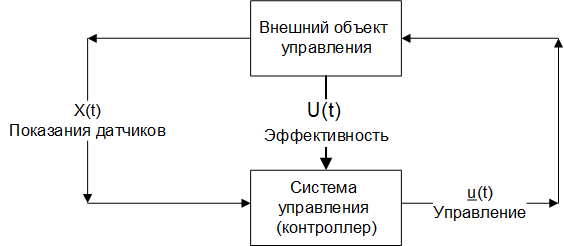
\includegraphics{images/intro/Система с подкрепляющим обучением.png}
    \caption{Система с подкрепляющим обучением}
    \label{fig:reinforce_learning_system}
\end{figure}

В настоящее время не только оборудование, применяемое на ОАО «Савушкин продукт», характеризуется очень высокой сложностью, но и технологические процессы также. Настройка параметров технологических линий требует наличия специалистов высокого уровня и занимает длительное время. Соответственно требования к качеству изготовления продукции очень высоки, так как от него напрямую зависит размер получаемой прибыли (выше качество – лучше потребительские характеристики товара – дольше срок хранения – более широкие возможности по географическому охвату рынка и т.д.). Нейроуправление позволяет повысить качество продукции за счет повышения эффективности управления, а также ускорить настройку параметров. Поэтому актуальной является задача применения нейроуправления для построения сложных управляющих систем на уровне АСУТП, которые были бы лишены недостатков, присущих используемым системам (на основе ПИД-регуляторов).
